\documentclass{beamer}
\usetheme{AnnArbor}



\usepackage[utf8]{inputenc}
\usepackage{amsthm}
\usepackage[slovak]{babel}
\usepackage{graphicx}


%[]

\title{\textbf{Rýchlokurz zlomkovej geniality\\}}
\date{}
\author{Roman Hudec}
\institute{Educat - vzdelávacie centrum}

\begin{document}
	
	\begin{frame}
		\titlepage
		
		\begin{center}
			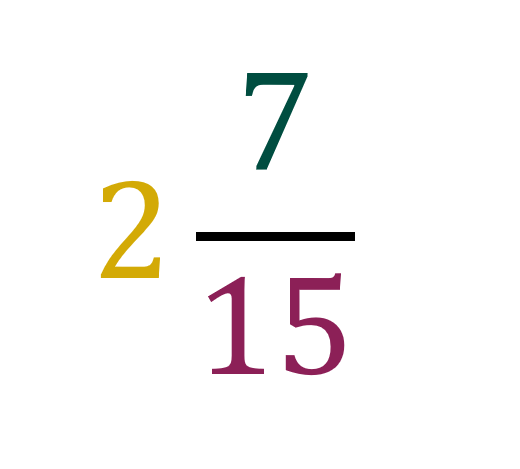
\includegraphics[width=4cm]{zlomok.png}
		\end{center}
		
	\end{frame}
	
	\begin{frame}
		\frametitle{Obsah}
		\tableofcontents
	\end{frame}
	
	
	\section{Čo sú to zlomky}
	
	\subsection{Definícia zlomkov a racionálnych čísel}
	
	\begin{frame}
		\begin{itemize}
			\frametitle{Zlomky}
			\item prirodzené čísla - $1, 2, 3, \dots$
			\item celé čísla - $\dots, -2, -1, 0, 1, 2, \dots$
		\end{itemize}
		
		\begin{definition}
			\textbf{Zlomok} je podiel 2 čísel.
		\end{definition}
	\end{frame}
\end{document}